\documentclass[10pt]{article}
\usepackage[margin=2cm]{geometry}
\usepackage[T1]{fontenc}
\usepackage{lmodern}
\usepackage{graphicx}
\usepackage{parskip}
\usepackage[hidelinks]{hyperref}
\graphicspath{{../01_reporte/figures/}}
\newcommand{\deltaMain}{$-$0.013}
\newcommand{\ciMain}{[$-$0.027, +0.002]}
\newcommand{\resBetter}{7 of 24}
\newcommand{\eegBetter}{17}
\newcommand{\resMainSubj}{0.761}
\newcommand{\eegMainSubj}{0.774}
\newcommand{\hypVerdict}{not supported}
\newcommand{\mainVerdict}{the interval includes zero, so the CNN on scalograms is not better than EEGNet on the raw signal; the two are statistically indistinguishable.}
\newcommand{\deltaInitial}{$-$0.005}
\newcommand{\deltaOldLr}{$-$0.024}
\newcommand{\ciOldLr}{[$-$0.037, $-$0.009]}
\newcommand{\oldLrSubj}{0.750}
\newcommand{\oldLrBetter}{5 of 24}
\newcommand{\deltaLrGain}{+0.011}
\newcommand{\ciLrGain}{[+0.005, +0.017]}
\newcommand{\lrGainBetter}{18 of 24}
\newcommand{\deltaCuda}{$-$0.007}
\newcommand{\ciCuda}{[$-$0.023, +0.009]}
\newcommand{\deltaCudaMps}{+0.006}
\newcommand{\ciCudaMps}{[$-$0.002, +0.013]}
\newcommand{\deltaCudaPair}{+0.000}
\newcommand{\ciCudaPair}{[$-$0.015, +0.017]}
\newcommand{\deltaStftCuda}{+0.006}
\newcommand{\ciStftCuda}{[$-$0.000, +0.012]}
\newcommand{\deltaScratch}{+0.015}
\newcommand{\ciScratch}{[+0.004, +0.025]}
\newcommand{\scratchSubj}{0.735}
\newcommand{\deltaStft}{+0.007}
\newcommand{\ciStft}{[$-$0.005, +0.019]}
\newcommand{\stftSubj}{0.755}
\newcommand{\deltaStftOld}{$-$0.001}
\newcommand{\ciStftOld}{[$-$0.010, +0.007]}
\newcommand{\stftVerdict}{indistinguishably}
\newcommand{\stftSentence}{the interval includes zero, so the choice of time--frequency transform does not measurably matter here.}
\newcommand{\stftShort}{makes no measurable difference}
\newcommand{\worstRange}{0.65 to 0.89 for EEGNet}
\newcommand{\worstSubjects}{22 (0.65, 51\% slow), 9 (0.69, 34\% slow), 31 (0.71, 21\% slow), 6 (0.71, 20\% slow)}
\newcommand{\condText}{0.791 (motion) vs.\ 0.782 (motionless) for EEGNet and 0.759 vs.\ 0.760 for ResNet18; a descriptive, not pre-registered, contrast.}
\newcommand{\agreePct}{86.2\%}
\newcommand{\disagree}{EEGNet 58.3\% vs.\ ResNet18 41.7\%}
\newcommand{\bothWrongSlow}{32.2\%}

\pagestyle{empty}

\begin{document}
{\Large\bfseries Images or raw signal? Decoding a subject-relative response state from pre-event EEG}\\[2pt]
Juan Pablo Acevedo Robles and Alberto Martinez Hernandez -- Team 8, Deep Learning final project -- one-page summary

\textbf{Thesis sub-objective.} Both authors infer subjective states from EEG that varies strongly between people: pain intensity (Alberto, quantification and standardization of pain) and trust in autonomous driving (Juan Pablo). The shared sub-objective is to determine which EEG representation generalizes best to \emph{unseen subjects} when the target is defined relative to each person. Because our own datasets are still being collected, a public sustained-attention driving dataset (Cao et al.\ 2019; 26 subjects, 18{,}087 windows) is the testbed. From 3\,s of Fz/Pz/Oz EEG before a lane deviation, we predict whether the response will be fast or slow relative to the subject's own session.

\textbf{Primary hypothesis.} A ResNet18 pretrained on ImageNet and fine-tuned on wavelet scalograms reaches higher balanced accuracy on unseen subjects than EEGNet on the raw signal, under the same data, folds, seeds, loss, early stopping, epoch cap and learning-rate search. Decision rule: mean per-subject $\Delta$ (ResNet18 $-$ EEGNet) $>0$ and its 95\% subject-bootstrap CI excludes 0.

\textbf{Principal result.} Not supported. With 5-fold subject-wise cross-validation $\times$ 3 seeds, EEGNet reaches \eegMainSubj{} per-subject balanced accuracy and ResNet18 \resMainSubj{}: $\Delta=\deltaMain$, 95\% CI \ciMain, a statistical tie. With the CNN at the edge of its first learning-rate grid ($10^{-4}$), EEGNet looked significantly better ($\deltaOldLr$); widening the grid removed that gap. Both networks clearly beat a band-power logistic regression (0.681), a time-on-task control (0.567) and permutation chance ($\approx$0.52, $p<0.001$). Ablations: ImageNet pretraining helps the CNN ($\deltaScratch$, CI \ciScratch); the wavelet vs.\ STFT choice \stftShort{} ($\deltaStft$, CI \ciStft).

\begin{center}
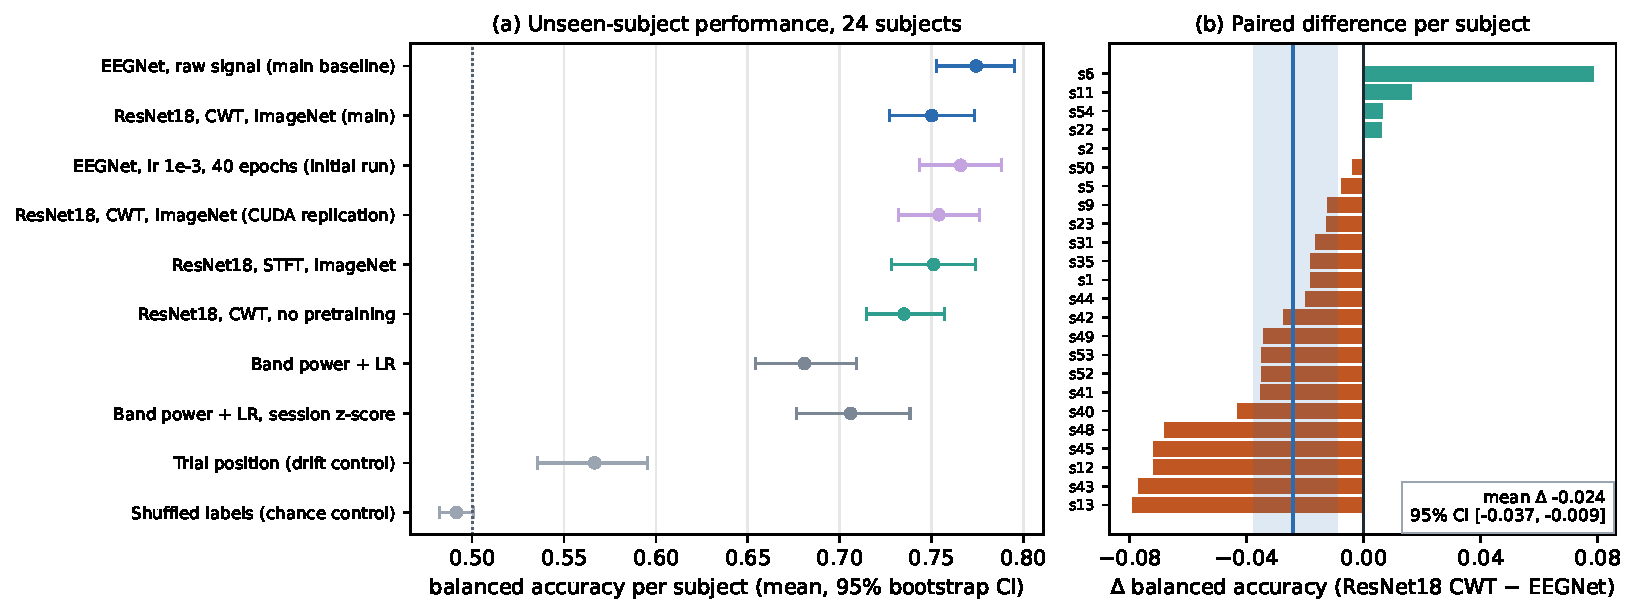
\includegraphics[width=0.8\textwidth]{fig_resultados}
\end{center}

\textbf{Key limitation.} A channel/band diagnostic shows that much of the information is low-frequency (delta) activity at Fz, which may be ocular rather than cortical, and 30--50\,Hz alone stays above chance (possible muscle activity). Labels are behavioral (reaction time), not an independent measure of drowsiness, and per-session normalization uses unlabeled data from the test session.

\textbf{Planned next step.} Alberto: apply the same protocol to his pain dataset once it reaches 40 subjects, predicting subject-relative pain intensity, starting from raw-signal EEGNet and adding ICA/EOG control for ocular and muscle artifacts. Juan Pablo: apply the pipeline to his CARLA trust dataset.
\end{document}
